\chapter{Concurrency}

\section{Introduction}

In this chapter, we introduce a new abstraction for a single running process:
that of a \textbf{thread}. Each thread is very much like a separate process,
except for one difference: they share the same address space and thus can
access the same data.\\

The state of a single thread is very similar to that of a process. It has a
program counter, a private set of registers. Two switch between two different 
threads, a \textbf{context switch} must occur. With processes we saved state to
a process control block (PCB); now, we need one or more \textbf{thread control
blocks (TCBs)}.\\

In multi-threaded processes, there are multiple stacks in a single process. 
This is thread local storage. This is destroyed after thread is finished. 
Better not to allocated memory here which is meant to be used later.

\begin{figure}[h!]
    \begin{center}
        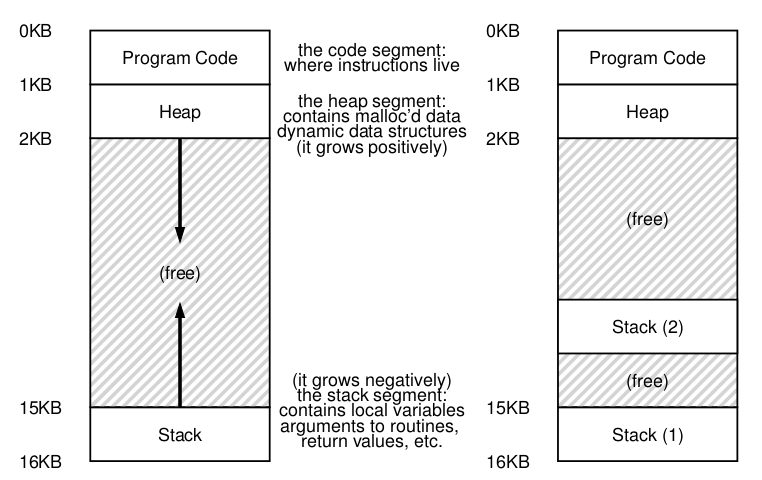
\includegraphics[width=8cm, height=4cm]{img/261.png}
        \caption{Single vs Multi Threaded Address Spaces}
    \end{center}
\end{figure}

\subsubsection{Why use threads?}

\begin{enumerate}
    \item \textbf{Parallelism:} Modern CPUs are multi-core. To take advantage of
        this fact.
    \item \textbf{Avoid blocking:} One thread does I/O while others does work.
\end{enumerate}

\subsection{Problem: Shared Data}

Lets take a simple example where two threads wish to update a single global
shared variable.

\begin{figure}[h!]
    \begin{center}
        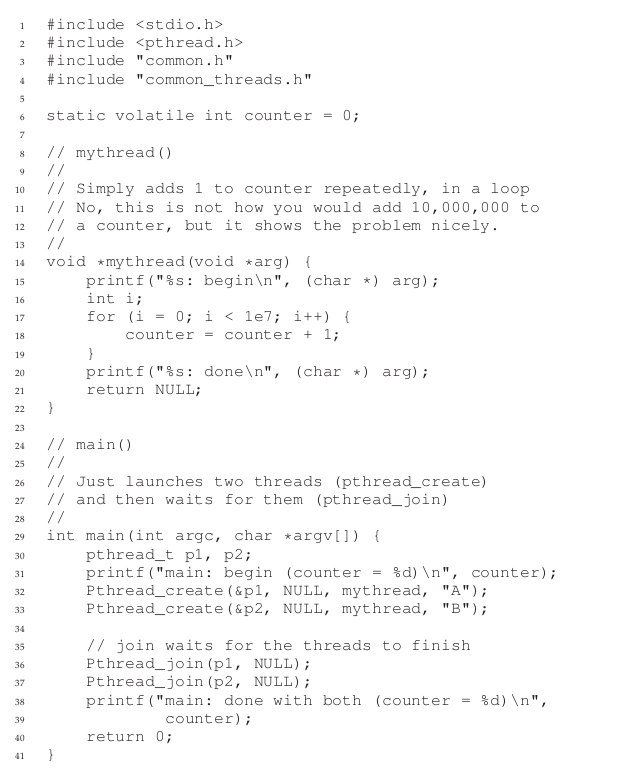
\includegraphics[width=9cm, height=7cm]{img/266.png}
        \caption{Sharing Data Problem}
    \end{center}
\end{figure}

(Here functions of pthread library with 'P' are same as with small 'p' with
some error checking)\\

When we run this code, we observe weird behavior. We get a wrong and weird
result each time.

\begin{figure}[h!]
    \begin{center}
        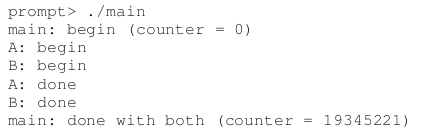
\includegraphics[width=5cm, height=2cm]{img/counterex.png}
        \caption{Wrong result}
    \end{center}
\end{figure}

The image below depicts why this happens:

\begin{figure}[h!]
    \begin{center}
        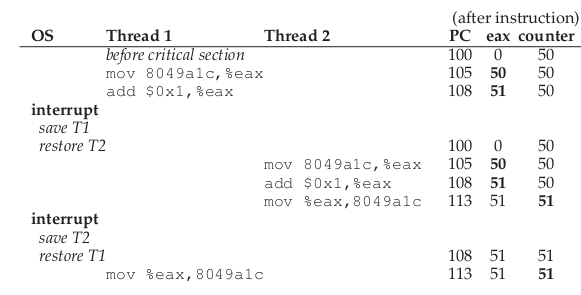
\includegraphics[width=7cm, height=5cm]{img/267.png}
        \caption{The Problem}
    \end{center}
\end{figure}

The problem demonstrated here is call a \textbf{race condition}. Each thread
tries to update the counter. The one that updates it later, actually updates it.
Because multiple threads executing the small piece of code can cause a race
condition, this piece is called a \textbf{critical section}. A critical section
is a piece of code that accesses a shared variable (or more generally, 
a shared resource) and must not be concurrently executed by more than one
thread.\\

What we want from this code is \textbf{mutual exclusion}. This propery 
gurrantees that only one thread will be in the critical section.\\

\textbf{Atmoic Operation:} A series of actions simply depicted by the 
sentence "All or nothing". An atomic operation is a powerful instruction in 
hardware which is or appears to be excuted at once on the cpu.\\

\subsection{Wish for Atomicity}

What we require to remove the data race in the problem above is that we want
the following instructions to be an atomic instruction:

\begin{figure}[h!]
    \begin{center}
        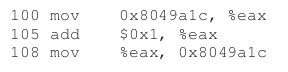
\includegraphics[width=4cm, height=2cm]{img/atomicex.png}
        \caption{Need for atomic instruction}
    \end{center}
\end{figure}

If we had a single instruction to do this, we could just use that instruction.
But in general case, we wont have a single instruction to build a concurrent
B-tree. Thus, we will use hardware support to get some \textbf{synchronization
primitives}.

\begin{tcolorbox}
    \begin{center}
        \textbf{The Crux: How to Support Synchronization}
    \end{center}  

    What support does the hardware need to provide in order to build useful
    synchronization primitives? What support do we need from OS? How can we
    build primitives correctly and efficently.
\end{tcolorbox}

\subsection{Another Problem: Waiting for Another}

Another common problem that arrises in concurrency is that of waiting for
another thread while it finishes. Thus concurrency is not only about making
shared resouces accessable but also about this waking/sleeping interaction.

\section{Locks}

We saw that one of the fundamental problems in concurrent programming: we would
like to execute a series of instructions atomically, but due to the presence of
interrupts on a single processor, we couldn't. Thus, we introduce \textbf{locks}.\\

We wrap a critical section around a critical section and it then executes it
as if it were a single atomic instruction.\\

\subsection{Basic Idea}

Lets assume our critical section is this:

$$
balance = balance + 1;
$$

Other critical sections are possible, but when we genearlize the principle, it
does not matter. To use a lock, we add it around the critical section as shown
in \ref{lockinit}

\begin{figure}[h!]
    \label{lockinit}
    \begin{center}
        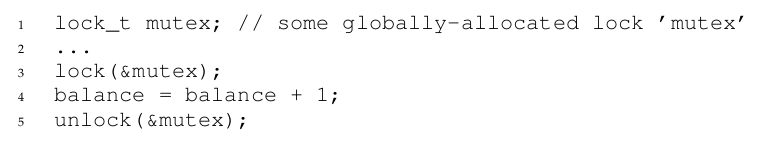
\includegraphics[width=7cm, height=3cm]{img/lockinit.png}
        \caption{Using a lock}
    \end{center}
\end{figure}

A lock is just a shared variable (must be initialized) that keeps track
if the critical section can be entered by the running thread. The lock variable
or "lock" for short, holds the state of lock at any time.\\

Calling $lock()$ tries to acquire the lock. If no other thread has the lock, 
the lock is acquired and the thread enters the critical section. If another
thread calls $lock()$ on the same lock variable, it will have to wait for the
other thread to release the lock first.\\

Once the owner of the lock calls $unlock()$, the lock is free again. If there
are waiting threads, one of the will acquire the lock.

\subsubsection{Pthread Locks}

The name that the POSIX library uses for a lock is a \textbf{mutex}, as it 
provides mutual exclusion between threads. Here is how you use it:

\begin{figure}[h!]
    \begin{center}
        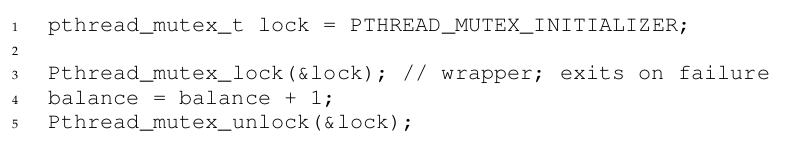
\includegraphics[width=8cm, height=3cm]{img/plocks.png}
        \caption{Using a POSIX lock}
    \end{center}
\end{figure}

As it can be seen, POSIX provides \textbf{fine-grained} approach i.e. allows 
different locks insted of one big lock over the critical section i.e. 
\textbf{course-grained} locking stratergy. 

\subsection{Building A Lock}

\begin{tcolorbox}
    \begin{center}
        The Crux: How To Build A Lock
    \end{center}

    How can we build an efficent lock? What hardware support is needed? What OS
    support is needed?
\end{tcolorbox}

\subsubsection{Evaluating a Lock}

\begin{enumerate}
    \item Correctness: Does it provide mutual exclusion?
    \item Fairness: Is the lock fair? i.e. Does each thread contending for the lock get
        and equal shot at acquiring it?
    \item Performance: How bad is the time overhead of using the lock
\end{enumerate}

\subsubsection{Controlling Interrupts}

An early solution to provide mutual exclusion was to disable interrupts for
critical sections of code; this solution was for single-processor systems.\\

The problem with this approach was that disablling interrupts is a \textit{privileged}
operation. This way is not secure as the user program can take control by
running an infinite loop inside the lock.\\

Another problem is that this approach is that it does not work on multi-processor
systems.\\

This approach is generally avoided. It is sometimes used by the OS to handle
is own kernal-based data structures. Trust issue is not a problem here as
the OS trusts itself.

\subsubsection{Just Using Loads/Stores}

Let's try building a simple lock by using a single flag variable:

\begin{figure}[h!]
    \begin{center}
        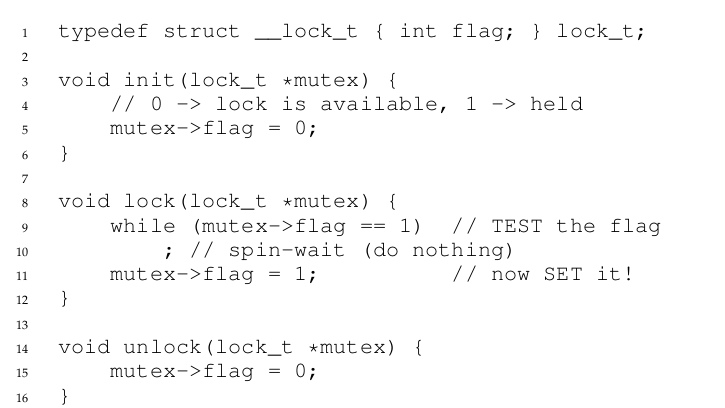
\includegraphics[width=7cm, height=4cm]{img/281.png}
        \caption{A Simple Flag}
    \end{center}
\end{figure}

This code has two problems.\\

\begin{enumerate}
    \item Correctness: This (\ref{282}) code does not provide mutual exclusion
        \begin{figure}[h!]
            \label{282}
            \begin{center}
                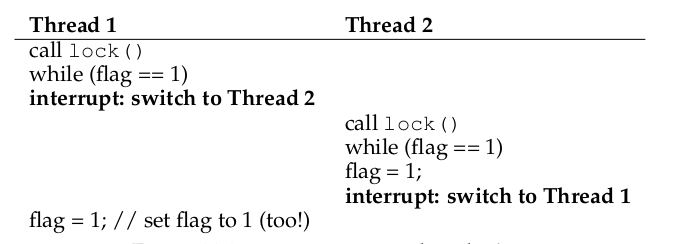
\includegraphics[width=7cm, height=3cm]{img/282.png}
                \caption{No Mutual Exclusion}
            \end{center}
        \end{figure}
    
    \item Performance: A thread waiting to acquire a lock which is already held
        endlessly checks the value of the flag in its time slice. This is known
        as \textbf{spin-waiting}. This wastes a lot of time while another thread
        could be running on the processor.
\end{enumerate}

\subsubsection{Working Sping Locks with Test-And-Set}

Today, all systems provide support for an atmoic intsruction to do a
\textbf{test-and-set} (or \textbf{atmoic exchange}). This (\ref{testandset})
instruction does this atomically.

\begin{figure}[h!]
    \label{testandset}
    \begin{center}
        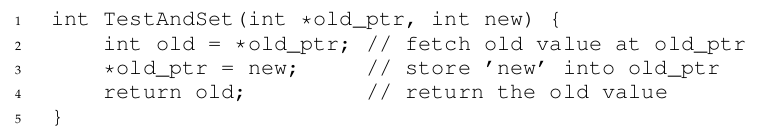
\includegraphics[width=8cm, height=2cm]{img/testandset.png}
        \caption{Test and Set}
    \end{center}
\end{figure}

This \textbf{atmoic} instruction is enough to build a \textbf{spin lock} as
shown in \ref{283}

\begin{figure}[h!]
    \label{283}
    \begin{center}
        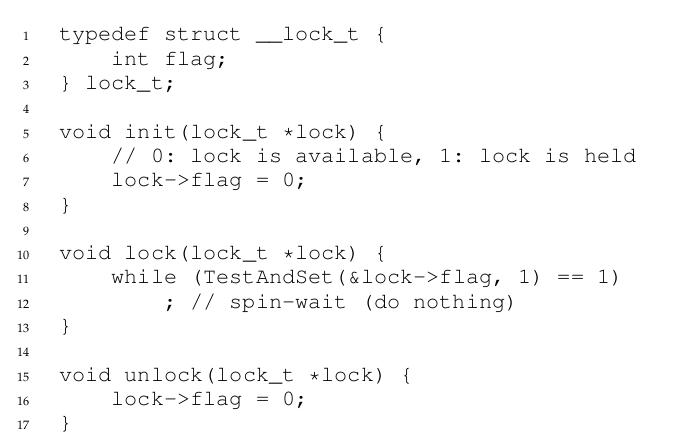
\includegraphics[width=7cm, height=5cm]{img/283.png}
        \caption{A Working Spin Lock}
    \end{center}
\end{figure}

\subsubsection{Evaluating Spin Locks}

\begin{enumerate}
    \item Correctness: Spin locks do provide mutual exclusion.
    \item Fairness: We cannot guarantee that a waiting thread will ever enter
        the critical section. Spin locks do not provide any fairness gurantees.
    \item Performance: Performance overhead can be very bad due to spin-waiting.
        Imagine the case where $N$ threads compete for a lock and one of them holds
        the lock. Now, lets say the schedular runs each of the $N - 1$ threads
        and tries to acquire the lock and thus waiting and wasting their time
        slice. This is very bad for performance.\\

        On multi processor systems, this isnt as bad assuming that number of
        threads is less than number of available CPUs because usually the critical
        section is very small and a thread running on another CPU can acquire
        it as soon as the owner of lock releases it.
\end{enumerate}

\subsubsection{Using Compare and Swap}

Another hardware primitive that some systems provide is the \textbf{compare-and-
swap} instruction. The C psudeocode for the instruction:

\begin{figure}[h!]
    \begin{center}
        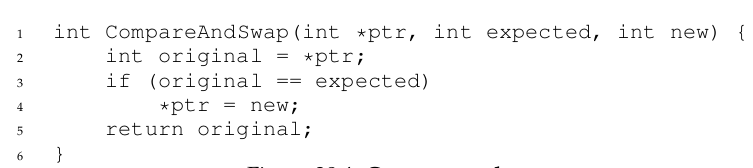
\includegraphics[width=7cm, height=3cm]{img/284.png}
        \caption{Compare and Swap}
    \end{center}
\end{figure}

To make a spin-lock using compare-and-swap, we can just replace the test-and-swap
instructon and modify a bit to do the same thing.

\subsubsection{Fetch And Add}

Another hardware primitive is the \textbf{fetch-and-add} instruction, which
atomically increments a value and returns it. Using this instruction we can make
a more interesting lock called a \textbf{ticket lock}.\\

Instead of a single value, this solution uses a ticket and turn variable in
combination to build a lock. The operation is simple: whn a thread wishes to
acquire the lock, it first does an atomic fetch-and-add on the ticket value;
that value is now considered this thread's "turn". The globally shared lock->turn
is then used to determine which thread's turn it is for a given thread. \\

The important difference between ticket locks and spin locks is that ticket
locks guarantee fairness while spin locks don't. Each threads progresses. We
can solve the problem of fairness using ticket locks. But they still have
the problem of spinning too much.

\begin{figure}[h!]
    \begin{center}
        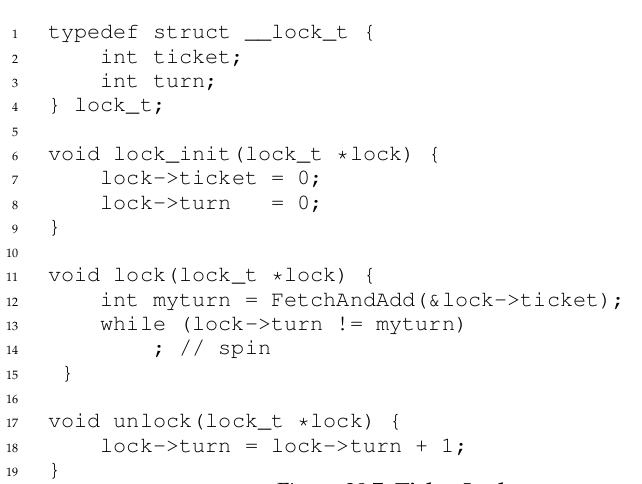
\includegraphics[width=8cm, height=5cm]{img/287.png}
        \caption{Ticket Locks}
    \end{center}
\end{figure}

\subsection{Reducing the amoung of Spining}

This part is related to making the locks more efficent by reducing the amount of
spining that they do.

\begin{tcolorbox}
    \begin{center}
        The Crux: How to Avoid Spining
    \end{center}

    How can we develop a lock that doesn't needlessly waste time spining on the
    CPU.
\end{tcolorbox}

We need OS support for this now.

\subsubsection{Using Yield}

In this approach we assume that the OS provides a primitive $yield()$ which a
thread can call when it wants to give up the CPU and let another thread run.
A thread can be in one of thethree states (running, read, or blocked); yield
is simply a system call that moves the caller from the \textbf{runnning} state
to the \textbf{ready} state. Thus allowing another thread to run. The yielding
thread essentially \textbf{descedules} itself.\\

This approach still has a problem of fairness and that of efficency as this 
approach leaves it all to the schedular which may do anything.

\subsubsection{Using Queues: Sleeping Instead of Spining}

The problem with previous approaches was they leave too much to chance (i.e.
behavior) of the schedular. This is not optimal as we have worst cases which
can occur easily. Thus, we must explicitly exert some control over which
threads acquires the lock after the current holder releases it.\\

We use an OS primitive: $park()$ which puts the calling thread to sleep and
$unpark()$ to wake a particular thread. Using this we can build a lock which
solves our problems as shown in \ref{289}.

\begin{figure}[h!]
    \label{289}
    \begin{center}
        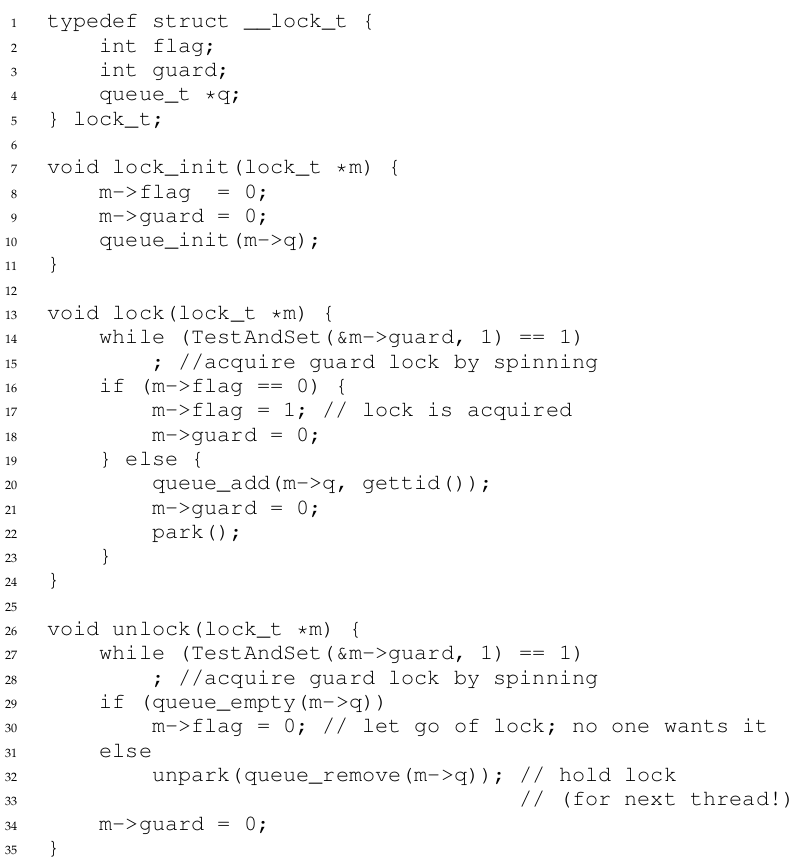
\includegraphics[width=8cm, height=9cm]{img/289.png}
        \caption{Locks with queues, test-and-set, yield, and wakeup}
    \end{center}
\end{figure}

We combine the old test-and-set idea with an explicit queue of lock waiters to
make a more efficent lock. Second, we use a queue to help control who gets the
lock next and thus avoid starvation.\\

This approach does not avoid spin-waiting; However the time spent spinning is
quite limited, and thus this approach may be reasonable.\\

There is one problem with this approach. there is a race conditon in the solution,
just before the call to $park()$. With the wrong timing, a thread
will be about to park, assuming that it should sleep until the lock is no longer
held. A switch at that time to another thread, (say a thread holding the lock)
coud lead to trouble, for example the owner of the lock releases the lock
and tries to unpark this thread and then the thread runs and parks itself.
It will now go into a sleep forever.\\

This problem can be solved by another OS primitive called $setpark()$. By
calling this routine, a thread can indicate it is \textit{about} to park.
If it then happens to be interrupted and another thread calls unpark
before park is actuall called, the subsquent park returns immediately instead
of sleeping. The code modification, inside the $lock()$, is quite small as shown
in \ref{setpark}

\begin{figure}[h!]
    \label{setpark}
    \begin{center}
        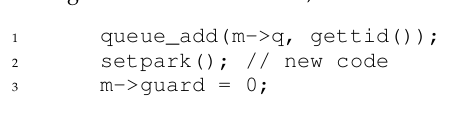
\includegraphics[width=7cm, height=2cm]{img/setpark.png}
        \caption{Using setpark}
    \end{center}
\end{figure}

Note: $park(), unpark(), setpark()$ are part of Solaris. Other OS may have 
different support.

\section{Condition Variables}

In many cases, a thread wishes to check whether a \textbf{condition} is true
before continuing its execution. For example, a parent thread might wish
to check wether a child thread has completed before continuing (often called a
$join()$).

The problem is shown in \ref{301}

\begin{figure}[h!]
    \label{301}
    \begin{center}
        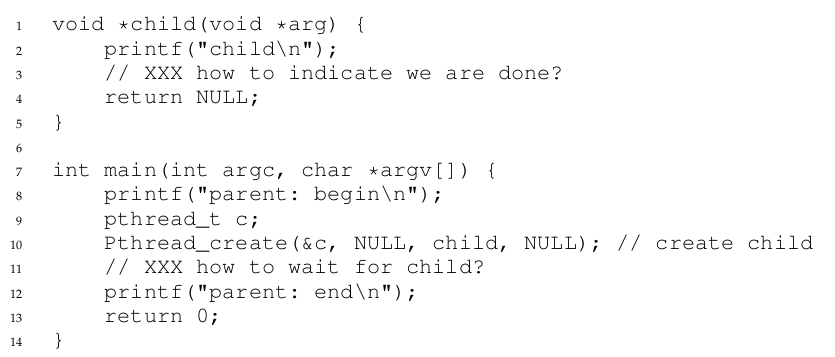
\includegraphics[width=7cm, height=5cm]{img/301.png}
        \caption{A Parent waiting for its Child}
    \end{center}
\end{figure}

We could try to use a shared variable and just spin. But this is very inefficent
as the parent spins and wastes CPU time as shown in \ref{302}

\begin{figure}[h!]
    \label{302}
    \begin{center}
        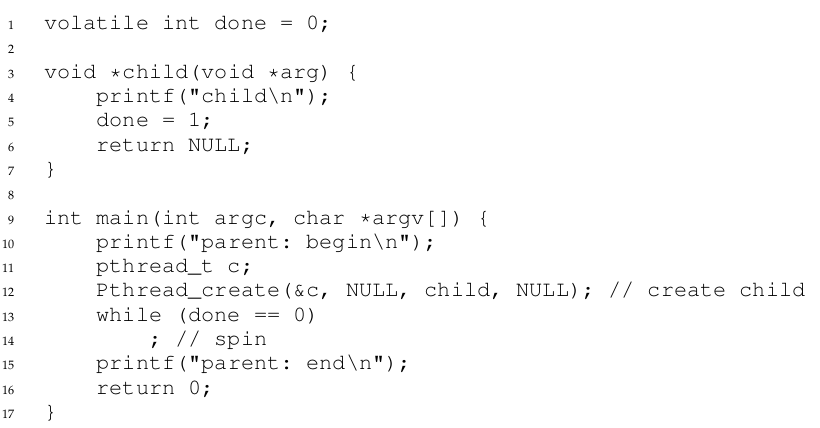
\includegraphics[width=7cm, height=6cm]{img/302.png}
        \caption{Spin based approach}
    \end{center}
\end{figure}

\begin{tcolorbox}
    \begin{center}
        The Crux: How To Wait For A Condition
    \end{center}

    In multi-threaded programs, it is often useful for a thread to wait for
    some condition to become true before proceeding. How should a thread wait for
    a condition?
\end{tcolorbox} 

A \textbf{condition variable} is an explicit queue that threads can put themselves on
when some state of execution (i.e., some \textbf{condition}) is not as desired
(by \textbf{waiting} on the condition). Some other thread, when it changes said
state, can then wake one (or more) of those waiting threads and thus allow them
to continue (by \textbf{signaling} on the condition).\\

\begin{figure}[h!]
    \begin{center}
        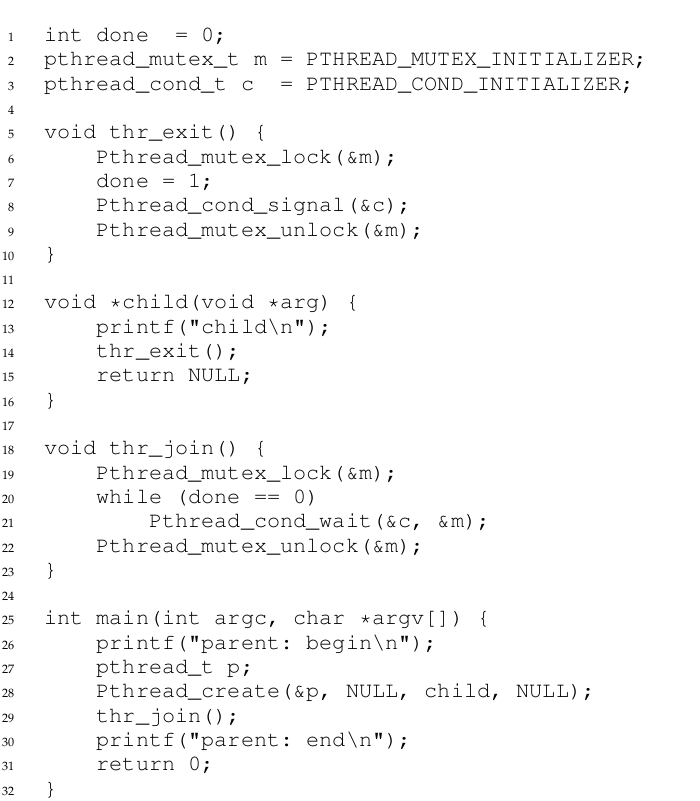
\includegraphics[width=7cm, height=8cm]{img/303.png}
        \caption{Using a condition variable to Solve Fork-Join problem}
    \end{center}
\end{figure} 

A thing to notice about $wait()$ call is that it also takes a lock as a paramter.
It assumes that this mutex is locked when $wait()$ is called. The responsibility
of $wait()$ is to release the lock and put the calling thread to sleep (atomically);
When the thread wakes up (after some thread has signaled it), it must re-acquire
the lock before returning to the caller.\\

Two things to better understand the code:

\begin{enumerate}
    \item Usage of the state variable $done$: Lets say we did not use this. The
        approach is broken then. The child may run and finish and signal immediatly
        after its created. And then the parent tries to wait and goes to a
        sleep forever.
    \item Usage of locks: This approach is again broken as after the parent 
        checks for $done == 0$, the child may signal before the wait is executed
        and thus the parent goes in an infinite sleep.
\end{enumerate}

Tip: Always hold the lock while signaling. A good general rule.\\

\section{The Bounded Buffer Problem}

Imagine one or more producer threads and one or more consumer threads. Producers 
generate data items and place them in a buffer; consumers grap said items from
the buffer and consume them in some way. Because the bounded buffer is a shared
resource, we require synchronized access to it.\\

Lets try to come up with a solution for only one item in the buffer.

\subsubsection{First solution}

\begin{figure}[h!]
    \begin{center}
        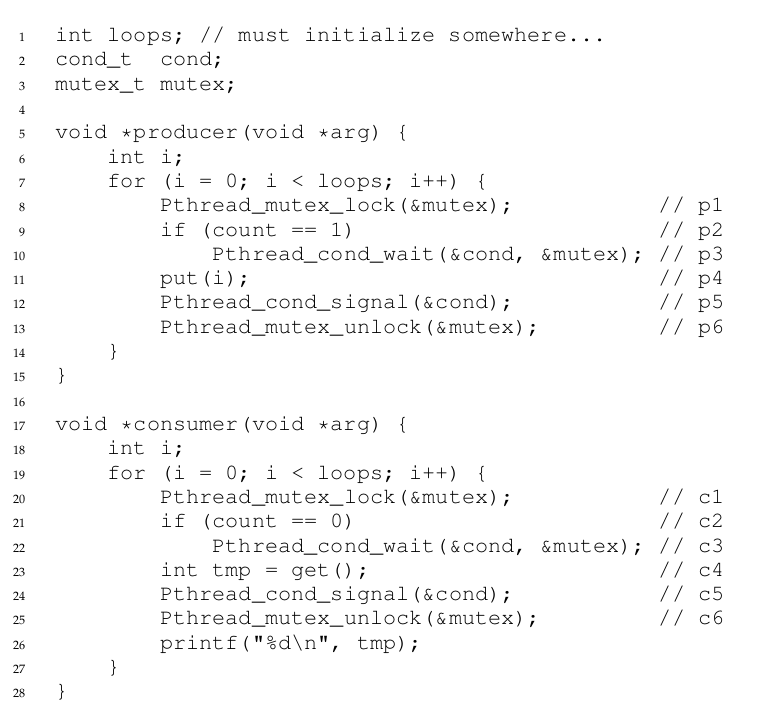
\includegraphics[width=7cm, height=8cm]{img/308.png}
        \caption{Single CV and If Statement}
    \end{center}
\end{figure}

With just a single consumer and single producer, this code works. But if we have
more than one of these threads, the solution breaks.\\

The problem is with the \textit{if} statement. Lets say we have
two running consumers $T_{c_1}, T_{c_2}$ and one producer $P$. $T_{c_1}$
is schedulded first and it sleeps. $P$ is schedulded after it and it signals
and now $T_{c_1}$ is in \textit{ready} queue. But now, $T_{c_2}$ runs.
$T_{c_2}$ runs and finishes and now $T_{c_1}$ runs and fails because there
is nothing in the buffer to take but it still tries to acquire something.\\

This problem arrises because the OS does not gurrantee that the thread
woken up will immediatly run. This reffered to as \textbf{Mesa semantics}.
The opposite behavior is called \textbf{Hoare semantics}, which provide
a harder guarantee that woken thread will run immediately upon being
woken up.

\subsubsection{Second solution}

The previous problem is easily fixable by converting the \textit{if} to a 
\textit{while} statement. Generally, in Mesa Semantics, its \textbf{always better
to use while loops}.\\

Another easy to see problem with this code is that there is only one condition
variable and it may signal the wrong thread. To fix that, we use two condition
variables instead.

\subsubsection{Full Producer/Consumer Solution}

\begin{figure}[h!]
    \begin{center}
        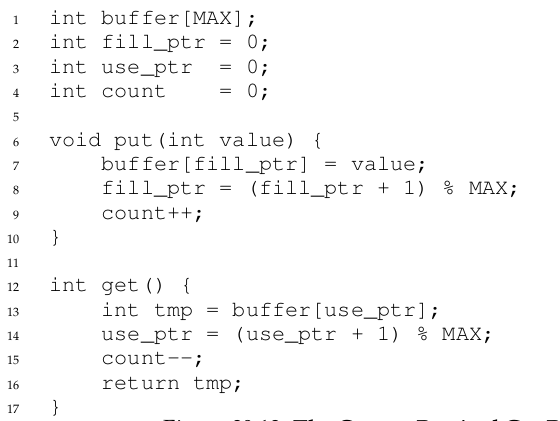
\includegraphics[width=7cm, height=7cm]{img/3013.png}
        \caption{The Correct Put and Get Routines}
    \end{center}
\end{figure}

\begin{figure}[h!]
    \begin{center}
        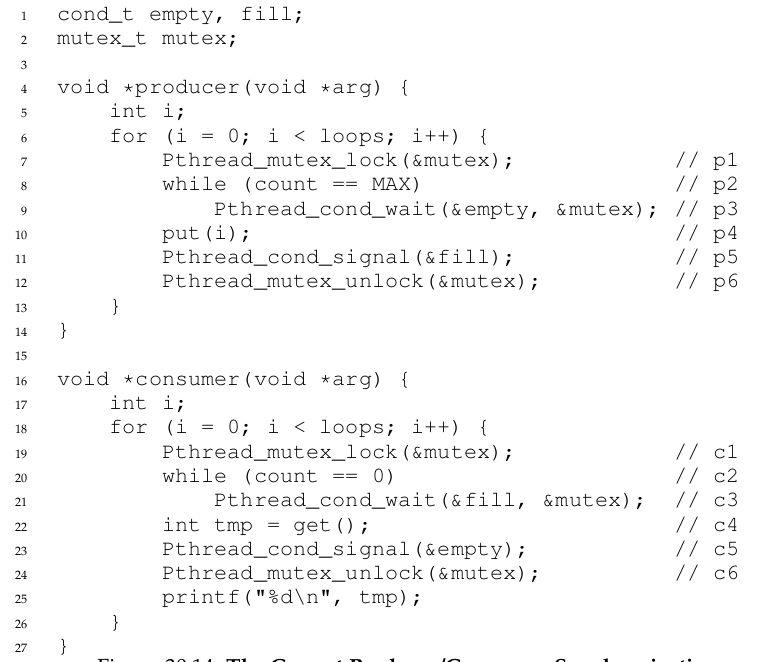
\includegraphics[width=7cm, height=9cm]{img/3014.png}
        \caption{Producer/Consumer Synchronization}
    \end{center}
\end{figure}
